\section{Programa de criptografía: CryptoPy}

Durante los últimos años, mi interés por la informática, la programación y el software libre ha ido creciendo. Comencé a familiarizarme con entornos Linux y a leer artículos relacionados con la ciberseguridad hasta descubrir el apasionante mundo de la criptografía.

Completamente escrito en lenguaje Python, CryptoPy recoge algunos de los métodos de cifrado más clásicos de la historia. El programa no está destinado a ser utilizado de forma real, sino más bien es un pequeño tributo al mundo de los códigos, las contraseñas, espías...

\begin{wrapfigure}{r}{0.5\linewidth}
	\centering
	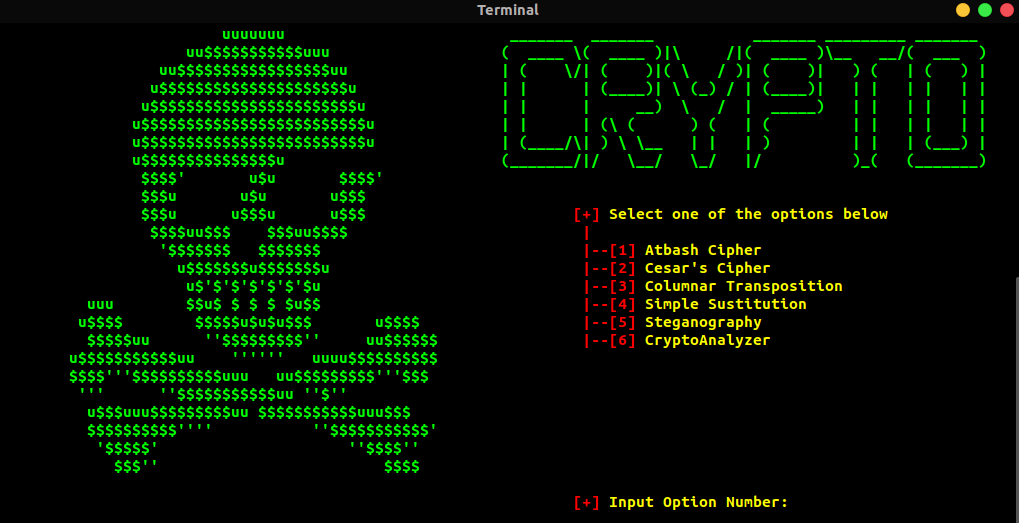
\includegraphics[width=1\textwidth]{cripto.png}
	\caption*{Pantalla principal del programa}
	\label{labelformat=empty}
\end{wrapfigure}